\documentclass{article}
\usepackage[margin=2.9cm]{geometry} % Adjust the margin size here
\usepackage{graphicx}
% \usepackage{multirow}
\usepackage{tabularx}
\usepackage{hyperref}
\usepackage{csquotes}
\usepackage{parnotes}
\usepackage{natbib} % for bibliography
\usepackage{listings} % for code
\usepackage{tablefootnote}
\usepackage{xcolor}
\definecolor{codegreen}{rgb}{0,0.6,0}
\definecolor{codegray}{rgb}{0.5,0.5,0.5}
\definecolor{codepurple}{rgb}{0.58,0,0.82}
\definecolor{backcolour}{rgb}{0.95,0.95,0.92}
% \usepackage{footnote}
\lstdefinestyle{PythonStyle}{
    language=Python,
    basicstyle=\small\ttfamily,
    keywordstyle=\color{magenta},
    commentstyle=\color{codegreen},
    stringstyle=\color{blue},
    numbers=left,
    numberstyle=\tiny\color{purple},
    stepnumber=1,
    frame=single,
    breaklines=true,
    breakatwhitespace=false,
    tabsize=4,
    showspaces=false,
    showstringspaces=false
}
\newenvironment{itquote}
  {\begin{displayquote}\itshape}
  {\end{displayquote}\ignorespacesafterend}


\title{\vspace{-1.3cm}Interim Results}
\author{Joel Pointon}
\date{\today}

\begin{document}

\maketitle
\section{Framework}\label{sec:inital_framework}
Given a set of documents (word documents, PDFs, Wikipedia pages), the proposed framework will chunk them into sections which contain sufficient context but are short enough to be processed by the model (and not use an excessive number of tokens). These sections are stored in a dataframe, along with the document name/section header, from which section embeddings are created. The same embedding model is used to also embed the student's question. The embedding model can be flexible:

\begin{enumerate}
    \item GPT offers its \texttt{text-embedding-ada-002} embedding model - it can process up to 4028 tokens
    \item A fine-tuned model of BERT \texttt{bert-base-nli-mean-tokens} seems to be the most appropriate - it is designed to capture two-way context but can only process 512 tokens
\end{enumerate}

Provided that both the documents of `knowledge' and the question are embedded using the same model, the embedding model need not necessarily be the same as the chatbot model itself. GPT's embedding model can process much longer contexts but has a small financial cost associated (Section \ref{sec:interim_summary}). However, it uses the \texttt{tiktoken} package which requires >= Python 3.8.

Once the embedding model has been chosen, the sections of `knowledge' can be embedded, along with each question, with their cosine similarity used to determine the top (n) relevant sections. These sections are fed into the chosen model, along with the student's question, and the AI provides a response (if the AI can't find an answer in the context provided then it should respond appropriately). This framework is shown in Figure \ref{fig:initial_framework}:

\begin{figure}[h!]
    \centering
    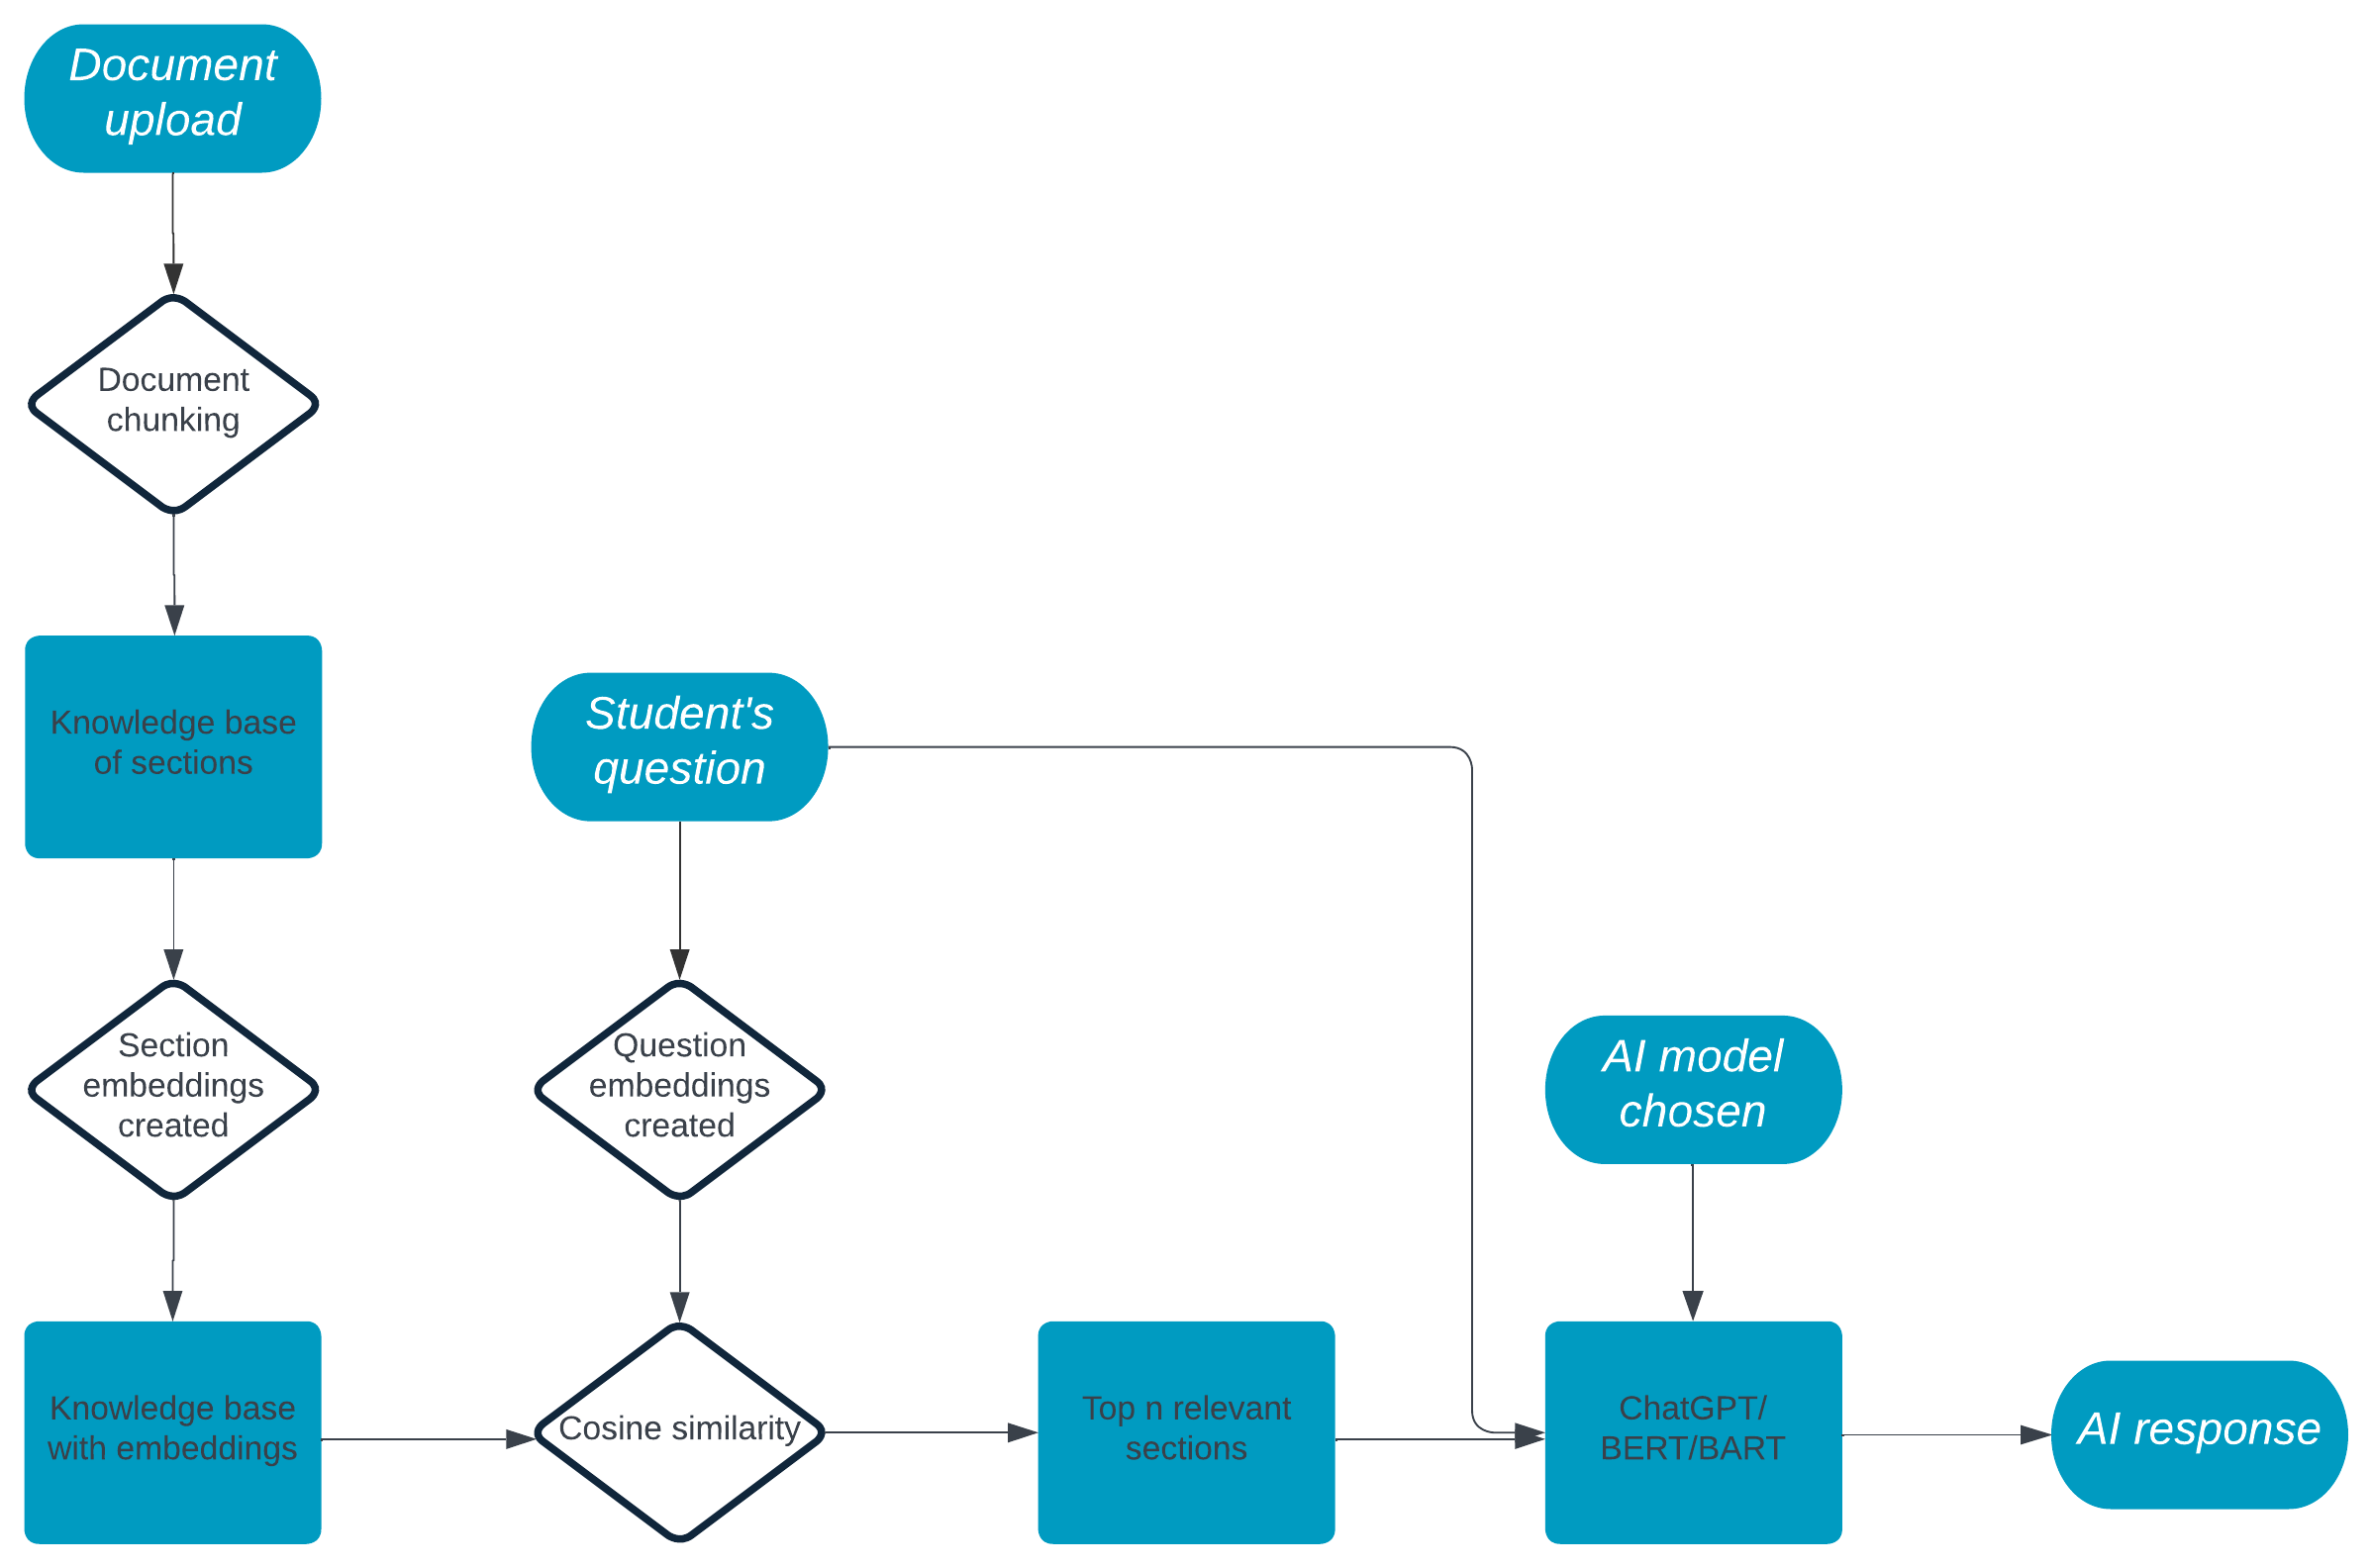
\includegraphics[width=0.8\textwidth]{images/framework.png}
    \caption{Proposed Chatbot Framework}
    \label{fig:initial_framework}
\end{figure}

\section{ChatGPT}

% Figure \ref{fig:initial_query_gpt} outlines how an instance of a custom class \texttt{ChatBot} can be created, from which one can ask questions based off the `knowledge' stored in \texttt{GPT\_KNOWLEDGE\_FILENAME} (which has been pre-processed and embedded, as per Section \ref{sec:inital_framework}).

% \begin{figure}[h]
%     \begin{lstlisting}[style=PythonStyle]
%         # Create an instance of the ChatBot class
%         CompVisionGPT = ChatBot("Computer Vision", 'assets/' + GPT_KNOWLEDGE_FILENAME)
    
%         # Ask the AI a question, and print out the sources used
%         print(Query.ask_bart('When did Universities begin teaching Computer Vision?', CompVisionGPT, show_source=True))
%     \end{lstlisting}
%     \caption{Creating and Querying a custom GPT Chatbot}
%     \label{fig:initial_query_gpt}
% \end{figure}

We will begin by discussing the efficacy of the GPT 3.5-turbo AI, which ChatGPT is based on, and can be accessed via OpenAI's API \citep{openAIAPI}. We can ask a question based on Wikipedia's Computer Vision page \citep{wikiCompVision}. The question `\textit{When did Universities begin teaching Computer Vision?}' has the highest cosine similarity with the following section in the `knowledge' database:

\begin{itquote}
    In the late 1960s, computer vision began at universities that were pioneering artificial intelligence. It was meant to mimic the human visual system, as a stepping stone to endowing robots with intelligent behavior. In 1966, it was believed that this could be achieved through a summer project, by attaching a camera to a computer and having it ``describe what it saw''.
    
    ...
    
    Researchers also realized that many of these mathematical concepts could be treated within the same optimization framework as regularization and Markov random fields.
\end{itquote}

The GPT chatbot responds with the following output:

\begin{itquote}
    Computer Vision began at universities in the late 1960s.

    To construct this answer, I used the following documents: 
    
    1. Wikipedia (Computer vision)->History:
    In the late 1960s, computer vision began at universities that were pioneering artificial intelligen...
    
    2. Wikipedia (Computer vision)->Definition:
    Computer vision is an interdisciplinary field that deals with how computers can be made to gain hig...
    
    ...
\end{itquote}

The correct answer of the `late 1960s' has been given in the first line, and has been written in natural language. This is the main strength of GPT-3.5: the stacked-decoder model makes it exceptional at writing natural, human-like responses. Furthermore, it has restricted its answer to using only the most relevant 5 sections within its knowledge base; we can easily print out the sections we fed into the chatbot so that students can verify the output and use the sources for further reading.

The main disadvantage is that the request is formatted as ``Use the below article on \{\texttt{chatbot\_topic}\} to answer the subsequent question. If the answer cannot be found in the article, write \{\texttt{answer\_not \_found\_message}\}.'', which means that the model is entirely reliant on GPT-3.5 understanding this request. As such, the model cannot guarantee that it will answer the request from the knowledge base (although my research shows that it is unlikely to deviate), or that it won't be tricked into answering outside of the provided sources/`knowledge'. A key reason for this is that it is not specifically trained to respond to this type of query, but instead to have high accuracy in zero- or few-shot tasks \citep{brown2020}. 

\section{BERT}
% Using a similar setup to GPT (but using BERT's embedding model, and limiting the number of tokens to 512 which leads to the \texttt{BERT\_KNOWLEDGE\_FILENAME} document), we can ask a query to the BERT AI using the code in Figure \ref{fig:initial_query_bert}:

% % BERT - extractive: softmax and tokens?

% \begin{figure}[h]
%     \begin{lstlisting}[style=PythonStyle]
%         # Create an instance of the ChatBot class
%         CompVisionBERT = ChatBot("Computer Vision", 'assets/' + BERT_KNOWLEDGE_FILENAME)
    
%         # Ask the AI a question, and print out the sources used
%         print(Query.ask_bert('When did universities begin teaching Computer Vision?', CompVisionBERT))
%     \end{lstlisting}
%     \caption{Creating and Querying a custom BERT Chatbot}
%     \label{fig:initial_query_bert}
% \end{figure}

Asking the same question to a BERT chatbot leads to the response below:

\begin{itquote}
    late 1960s
    
    To construct this answer, I used the following documents (specifically section 1): 
    
    1. Wikipedia (Computer vision)->History:
    In the late 1960s, computer vision began at universities that were pioneering artificial intelligen...
    
    2. Wikipedia (Computer vision)->Definition:
    Computer vision is an interdisciplinary field that deals with how computers can be made to gain hig...

    ...
\end{itquote}

As can be seen, this model is purely `extractive' - it can only find the most probable start token (word) and most probable end token and display the words within these two points. As such, it cannot generate its own content which sounds realistic but is false. It can, however, provide incorrect answers if it thinks it has found an answer and displays some text within its knowledge which is incorrect. This is unlikely to occur, as \citet{devlin2019bert} argues that BERT overcomes GPT's limitations in only considering left-to-right context by taking into account bidirectional context. Consequently, BERT's architecture is fine-tuned on question answering, with its gradient updates taking into account both directions of context, unlike GPT. BERT is therefore designed to better understand the context of the question and performs very well on many question-answering benchmarks \citep{devlin2019bert}. 

The proposed framework utilises the open-source nature of BERT, which means that the model can state which section/source it retrieved the answer from (``specifically section 1''), because it takes one section at a time and searches the most relevant section to find an answer first, before moving onto the next relevant section. Providing the exact source used improves the ability of students to quickly find additional relevant information and conduct wider reading efficiently. 

\section{BART}
BART is a generative model similar to GPT, but used a combination of bidirectional encoders and autoregressive decoders \citep{lewis2019bart}. While it can provide relatively human-like responses, it can provide answers that are not limited to the `knowledge' it is provided, and answer based on information it was trained on. Furthermore, it is limited to 1024 tokens, and so cannot process as much context at GPT. By using the GPT embeddings to find the most relevant documents, we can ask the same question and feed the same documents that we did to GPT. The response using BART is below:

\begin{itquote}
    Computer vision has been around for a long time, but it wasn't until the 1960s and 1970s that it really took off as a field of study. Prior to that, computer vision had been used in other fields, such as photogrammetry (the study of how light interacts with different parts of the human body) and stereoscopic photography. In the mid-1960s, there was a lot of interest in computers being able to ``see'' 3D objects, which is what we now think of as ``computer vision''. The idea was that computers would be able to figure out what an object looked like by looking at

    To construct this answer, I used the following documents : 
    
    1. Wikipedia (Computer vision)->History:
    In the late 1960s, computer vision began at universities that were pioneering artificial intelligen...
    
    2. Wikipedia (Computer vision)->Definition:
    Computer vision is an interdisciplinary field that deals with how computers can be made to gain hig...
    
   ...
\end{itquote}

There are several issues with this response. Firstly, it hasn't restricted the response to the `knowledge' it was provided. The Wikipedia page it was provided doesn't reference stereoscopic photography and doesn't talk about interest in the ability of computers to ``see'' 3D objects. Secondly, the response has some content which isn't relevant to the initial query. It is also important to note that other examples during my research saw very long answers which were repetitive and of poor quality, such as the one below:

\begin{itquote}
    Computer vision is the study of how computers can understand images. It is a field of study that is very much in the realm of engineering. It is a field of study that is very much in the realm of science. It is a field of study that is very much in the realm of mathematics. It is a field of study that is very much in the realm of science.....
\end{itquote}

To counteract this, a repetition penalty can be entered, along with a maximum response length, but this leads to the third issue in the model: the truncated ending. The above response finished with ``by looking at'', without finishing the sentence. Overall, the currently used model is poor. It could potentially be improved with additional fine-tuning, but this would require a large, reliable dataset to improve the model beyond the fine-tuning already conducted \citep{Blagojevic}.

\section{Summary}\label{sec:interim_summary}

Open source-extractive models such as BERT can specify \textit{exactly} which section of its knowledge it used to answer a question, and excels at providing exact responses from the text. This benefits students by narrowing the sources required for further reading. Furthermore, BERT's responses are unlikely to provide answers which seem accurate but are completely false - though this is because the model does not respond in a human-like format. While BART can provide more natural-sounding responses, its response quality is much poorer than GPT's, and the model often uses its training data to provide answers, rather than restricting responses to the context provided.

I conclude that the choice of model depends on the value placed on the quality of human-like responses. This backs up the findings of \citet{brown2020}, who noted that using the SuperGLUE benchmark (a standardized collection of datasets), GPT-3 outperforms BERT's average of 69.0 by achieving a score of 71.8 using few-shot learning. However, their results show that GPT-3 performs relatively poorly compared to SOTA levels for SQuADv2 (69.8 vs 93.0 F1 score) and other reading comprehension tasks. This is likely due to the training methods used with GPT, which has not been fine-tuned on these datasets and is designed to generate content in response to zero- or few-shot tasks (such as conducting arithmetic or writing articles which are indistinguishable from human form), rather than provide precise answers. However, this level of performance comes at a cost.

The superior performance of GPT comes at a higher cost than open-source models. As shown in Table \ref{tab:initial_cost_comparison}, BERT and BART have no outright cost for usage (aside from the running costs: electricity, hardware, setup time etc.). While each query using GPT is very cheap, it is cumulatively likely to cost several hundred pounds per year for each module that uses it, which might be unattainable for several departments. Additionally, departments would need to justify that this model is sufficiently more robust, reliable, and beneficial than ChatGPT (which is currently free). Note that there is also a very small cost each time a query embedding is requested (\$0.0004/1,000 tokens), but this is negligible compared the cost of asking GPT for an answer, as the number of tokens per query is very small (<50).

\begin{table}[h!]
    \centering
    \caption{Comparison of Estimated AI Costs}
    \begin{tabularx}{0.8\textwidth}{p{3.5cm}|>{\raggedright\arraybackslash}X|>{\raggedright\arraybackslash}X|>{\raggedright\arraybackslash}X}
        \hline
        \textbf{Model} & \textbf{Cost per query\parnote{Estimated cost using based on each query using 2000 tokens}} & \textbf{Cost per student\parnote{Estimated cost using based on 100 queries per student}} & \textbf{Cost per module\parnote{Estimated cost using based on 300 students in a module}}\\
        \hline
        GPT: \texttt{3.5-turbo} & \$0.004 & \$0.40 & \$120\parnote{Excluding the small cost of embedding students' questions} \\
        \hline
        BERT: \texttt{deepset/bert-base-cased-squad2} & \$0.00 & \$0.00 & \$0 \\
        \hline
        BART: \texttt{vblagoje/bart\_lfqa} & \$0.00 & \$0.00 & \$0 \\
        \hline
    \end{tabularx}
    \parnotes
    % \vspace{-25pt}
    \label{tab:initial_cost_comparison}
\end{table}

All models have their merits, but GPT is easily the most impressive model, excelling at providing human-like responses, and limiting its answers to the sources provided - it's a classic case of `you get what you pay for'.

\section{Future Research}
Based on the above findings, there are a number of avenues to explore, with five potential options outlined below:
\begin{enumerate}
    \item The `chunking' of documents and how to efficiently split documents into reasonably-sized sections. This is particularly challenging for PDFs because section titles can often be different sizes and they are never identified with 100\% certainty, because section headers can only be estimated using text size/colour/bold (typography). 
    \item Expanding the document types the chatbot can process. Currently only word documents, PDFs, and Wikipedia pages can be processed. Expanding this to other document types, such as general websites could be useful for some modules.
    \item The creation of a user interface. Creating a way that students can interact with the chatbot is a fundamental part of how accessible the framework is.
    \item Adapt the framework to include RoBERTa, an improved, fine-tuned version of BERT - but this would still only provide extractive responses, and not generative ones.
    \item Testing the chatbots on students. It would be interesting to provide an evaluation of how the different AIs perform and how they are reviewed by a selection of students. However, testing that chatbots on students has ethical considerations and could be difficult to arrange at short notice.
\end{enumerate}

Creating a UI for the model seems the preferred option due to its interesting applications and ability to bring a `completeness' to the project. Testing the chatbots on students would be worthwhile to have a more robust understanding of potential risks/inaccuracies, but it is clear that GPT is the best option if affordable, and a UI would be preferential before conducting research on potential users. Therefore, while all options are worthy of exploration, creating a UI seems the most beneficial.

\bibliographystyle{ecta} %for harvard
\bibliography{paper/bibliography/bibliography}

\end{document}
